%%%%%%%%%%%%%%%%%%%%%%%%%%%%%%%%%%%%%%%%%%%%%%%%%%%%%%%%%%%%%%%%%%%%%%%%%%%%%%%%
%2345678901234567890123456789012345678901234567890123456789012345678901234567890
%        1         2         3         4         5         6         7         8

\documentclass[letterpaper, 10 pt, conference]{ieeeconf}  % Comment this line out if you need a4paper

%\documentclass[a4paper, 10pt, conference]{ieeeconf}      % Use this line for a4 paper

\IEEEoverridecommandlockouts                              % This command is only needed if
                                                          % you want to use the \thanks command

\overrideIEEEmargins                                      % Needed to meet printer requirements.

%In case you encounter the following error:
%Error 1010 The PDF file may be corrupt (unable to open PDF file) OR
%Error 1000 An error occurred while parsing a contents stream. Unable to analyze the PDF file.
%This is a known problem with pdfLaTeX conversion filter. The file cannot be opened with acrobat reader
%Please use one of the alternatives below to circumvent this error by uncommenting one or the other
%\pdfobjcompresslevel=0
%\pdfminorversion=4

% See the \addtolength command later in the file to balance the column lengths
% on the last page of the document

% The following packages can be found on http:\\www.ctan.org
%\usepackage{graphics} % for pdf, bitmapped graphics files
%\usepackage{epsfig} % for postscript graphics files
%\usepackage{mathptmx} % assumes new font selection scheme installed
%\usepackage{times} % assumes new font selection scheme installed
\usepackage{amsmath} % assumes amsmath package installed
%\usepackage{amssymb}  % assumes amsmath package installed
\usepackage{csquotes}
\usepackage{hyperref}
\usepackage{stmaryrd}
\usepackage[svgnames,dvipsnames]{xcolor}
\definecolor{shadeGray}{rgb}{0.9,0.95,0.95}
\usepackage[bordercolor=red, backgroundcolor=shadeGray, linecolor=red, textwidth=0.8in, textsize=footnotesize]{todonotes}
\usepackage{listings}
\usepackage{tikz}
\usepackage{pgfplots}
\usepackage{subfig}
\usepackage{paralist}
\lstdefinestyle{corelang}{
  %frame=tb,
  %rulesepcolor=\color{gray},
  rulecolor=\color{gray},
  morekeywords={
  repeat, times, foreach, visit, pick, drop, containing, strict
  },%in,
  sensitive=true,
  morecomment=[l]{//},
  morecomment=[s]{/*}{*/},
  commentstyle=\color{gray},
  showstringspaces=false,
  columns=fullflexible,
  mathescape=true,
  numberstyle=\tiny,
  basicstyle=\footnotesize\ttfamily,
  numbersep=5pt,
  stepnumber=2,
  numbers=none,                   % where to put the line-numbers
  morestring=[b]"
}
\lstset{style=corelang}
\usepackage[T1]{fontenc}  % this is necessary for beramo to work
\usepackage[scaled=0.80]{beramono}  % our monospace font

\newcommand{\sem}[2]{\llbracket \texttt{#1}\rrbracket ::= #2}

\title{\LARGE \bf
LASRE looking for a new name
}


\author{Albert Author$^{1}$ and Bernard D. Researcher$^{2}$% <-this % stops a space
\thanks{*This work was not supported by any organization}% <-this % stops a space
\thanks{$^{1}$Albert Author is with Faculty of Electrical Engineering, Mathematics and Computer Science,
        University of Twente, 7500 AE Enschede, The Netherlands
        {\tt\small albert.author@papercept.net}}%
\thanks{$^{2}$Bernard D. Researcheris with the Department of Electrical Engineering, Wright State University,
        Dayton, OH 45435, USA
        {\tt\small b.d.researcher@ieee.org}}%
}


\begin{document}



\maketitle
\thispagestyle{empty}
\pagestyle{empty}


%%%%%%%%%%%%%%%%%%%%%%%%%%%%%%%%%%%%%%%%%%%%%%%%%%%%%%%%%%%%%%%%%%%%%%%%%%%%%%%%
\begin{abstract}

We present \tool, a natural language interface to describing 
high level task specifications for robots which can be automatically
compiled into correct-by-construction reactive plans.
Internally, \tool defines a core language for task planning that includes
predicates on the world, fluents (robot actions) that modify the state of the world, 
as well as temporal constraints.
A planner takes a program in the core language and automatically generates a (possibly reactive)
plan.
Externally, \tool provides a natural language interface to users and a visual feedback
mechanism.
It uses semantic parsing techniques from natural language to compile user utterances into
programs in the core language.
Then, it provides immediate visual feedback by executing the automatically constructed plan in the world
and allows the user to select between potentially ambiguous interpretations.
Unlike other systems, \tool enables natural language interactions while maintaining the expressive
power of a programming language. 
Additionally, the system learns through repeated interactions and generalizes learnt concepts.
We show through an initial user study that natural language interactions and generalization
can considerably ease the description of tasks, and moreover, over time,
users employ more and more defined concepts, not necesarily defiend by themselves. 

\end{abstract}


%%%%%%%%%%%%%%%%%%%%%%%%%%%%%%%%%%%%%%%%%%%%%%%%%%%%%%%%%%%%%%%%%%%%%%%%%%%%%%%%

\section{INTRODUCTION}



\section{Core Language}
Interesting core-language examples

\begin{itemize}
	\item drop an item to any field that contains both red item and circle-shaped item (can be the same item): \textit{foreach point in \{world containing item has color red\} and \{world containing item has shape circle\} \{visit point; drop item\}}
	\item if possible, form a horizontal line on the floor out of all items robot currently has and starting at robot's current position: \textit{strict \{while robot has item \{drop item; move right\}\}; strict \{while robot has item \{drop item; move left\}\}}
	\item keep bringing circle-shaped items to room1 until there is a red item in room1: \textit{while not \{ item has color red at room1\} \{visit \{world containing item has shape circle\} minus room1; pick item has shape circle; visit room1; drop item has shape circle\}}

\end{itemize}

\section{Naturalization of the Language}


\subsection{Semantic Parsing}


\subsection{Example}


The task of putting all items of different colors to different rooms looks in the core language like this \\
\begin{displayquote}
 \textit{foreach point in world containing item has color red \{ visit point; pick every item has color red\}; visit room1; drop every item has color red; foreach point in world containing item has color green \{ visit point; pick every item has color green\}; visit room2; drop every item has color green; foreach point in world containing item has color blue \{ visit point; pick every item has color blue\}; visit room3; drop every item has color blue; foreach point in world containing item has color yellow \{ visit point; pick every item has color yellow\}; visit room4; drop every item has color yellow} 
\end{displayquote} 
 The same task could be accomplished using naturalization with 
\begin{displayquote} 
 \textit{red to room1; green to room2; blue to room3; yellow to room4}
\end{displayquote} 
  with a single definition of \textit{red to room1} as
  \begin{displayquote}
  \textit{foreach point in world containing item has color red \{ visit point; pick every item has color red\}; visit room1; drop every item has color red}
  \end{displayquote}.
  If the next thing would be to put all items of different shapes to different rooms, it would again be possible to do it by 
\begin{displayquote}  
   \textit{ triangle to room1; circle to room2; square to room3}
   \end{displayquote}

\section{Evaluation}


We performed a number of trials of the system under different conditions.We ultimately want to create a system that people with different levels of proficiency in the core language would use. Users could range from \emph{expert users}  (the ones that would define new commands to make the communication to the robot simpler) all the way to ones whod don't know the language at all, but take advantage of commands that \emph{sound as if they should work}, defined by the other users of the system.
In the evaluation performed we were interested in two properties: whether or not users are inclined to define new commands that make their work easier and how much they are able to benefit from other people's definitions (without knowing them in advance).  The first property resembles defining a function in a programming language (except that in XnameX the system tries to generalize the definition from an example). The second property describes how much closer the system gets to pure natural-language interface if there is a number of active expert users. The assumption is that people will have similar (linguistic) ideas on how to express similar commands and that's why they don't have to be aware of existing definitions.
\paragraph*{\textbf{Setup}} We created a list of 21 tasks. The tasks levels ranged from easy (e.g.\  \emph{get one green square}) to difficult (e.g.\ \emph{bring all red items to a room that contains a yellow square}\footnote{the list of all tasks is available at \url{URL TO LIST OF TASKS}}). Fourteen participants (with prior programming experience, but without any knowledge of the system) were split into groups $A$ (4 members), $B$ (6 members) and $C$ (3 members). Group $A$ was only allowed to use the core language, group $B$ could additionally define their own concepts. Finally, group $C$ had access to concepts defined by two expert users as well as by other participants in the experiment. Participants were instructed to solve tasks as they see fit - not necessarily in the most general way. At the start of the experiment each group went through the core language tutorial\footnote{tutorial is available at \url{TUTORIALURL}}. Each group had half an hour to go through the tutorial and the average time needed to solve all tasks was one and half hour (but there was no deadline set). For each participant we measured the number of accepted commands (the ones that are part of either the core-language or that are induced by naturalization), number of words used to finish all tasks, number of defined concepts, number of used induced commands - with a distinction of whether they are used by that participant or by other participant.
\paragraph*{\textbf{Difficulty of learning the core language}} The average number of successful queries in group $A$ was 75\%. Additionally, judging from the feedback by participants and the questions they were asking during the experiment, we conclude that learning the core-language in half an hour is not an easy task. (However simple we might have thought the language was.) It is also interesting to notice that there were big differences among participants - from 63\% to 90\% of successful commands.
\paragraph*{\textbf{Naturalization makes work easier}} When comparing groups $B$ and $C$ to group $A$, it is clear that the participants who were able to use naturalization end up with less work in terms of total number of tokens needed to finish the tasks. Specifically, the average number of total tokens in the successful queries for groups $B$ and $C$ is 1156, while for the group $A$ it is 1765. This takes into account all tokens, also the ones from unsuccessful commands. (Some number of unsuccessful commands by groups that use naturalization comes from trying out commands they believed might be defined by others.) If we filter out the unsuccessful commands, the result becomes 738 compared to 1287 (i.e.\ improvement of 43\% with respect to the usage of core language only).  The averages hint that with naturalization reduces users' effort. It is important to emphasize that individual performance of participants in a single group varies significantly. To give a whole picture, the results per participant are shown in Figure \ref{fig:numTokens}.
\paragraph*{\textbf{Relying on the concepts defined by others}} It is interesting to observe results by group $C$. The participants adopted wildly different strategies. While they were on average more likely to use induced language over the core language (43 commands in comparison to 35 commands), it was only one participant who relied primarily on induced language, while for the other two the ratio was a little bit in favor of core language (as shown in Figure \ref{fig:groupCCoreVSInduced}). The main point of the experiment for group $C$ was to see if the existence of previously defined concept is helpful. First thing to notice is that participants were using concepts defined by others (Figure \ref{fig:groupCRulesInducedBySelfVsOthers}). The numbers differ among participants significantly. By closer look at the kinds of commands issued by each participant, we see that these differences stem from their individual styles: participant $C2$ chose to try small building blocks that matched the style of two expert users whose definitions were available to group $C$. Participant $C3$, on the other hand, used commands similar to the core language. That didn't find a match among predefined rules. \footnote{All commands by all experiment participants are available at \url{URLFORALLDATA}}
\paragraph*{\textbf{Types of defined concepts}} 
Upon closer inspection of the concepts the participants defined, we see that a majority falls into two categories: 
\begin{inparaenum}[(1)]
\item simplifying individual commands and
\item defining functions 
\end{inparaenum}.

Examples for the first case are  
\textit{pick green square} defined as \textit{pick item has color green} and 
\text{\textit{visit empty space}} defined as \textit{visit world minus {world containing item}}

For the second case a simple example is 
\textit{visit both triangle and green
} defined as \textit{ visit { { world containing item has shape triangle } and { world containing item has color green } }}. There were also function definitions that involved previous function definitions, such as \textit{line red} being defined \textit{as fetch all red; while { robot has item } { drop item ; move left }}.  Another noticeable phenomenon was that group C was defining many concepts that were previously defined by others. The reason were small variations in the definitions (e.g.\ \emph{pick red} vs.\ \emph{take a red} vs.\ \emph{take a red item}). 


 


\begin{figure}[t!]
		
		\resizebox{\linewidth}{!}{
		\centering
				\begin{tikzpicture}
				\begin{axis}[
				ticklabel style = {font=\tiny},
				    ybar,
				    bar width = 3,
				    area legend,
				    %enlargelimits=0.15,
				    legend style={at={(0.5,-0.15)},
				      anchor=north,legend columns=-1},
				    ylabel={\# tokens},
				    symbolic x coords={A1, A2, A3, A4, B1,B2,B3,B4,B5,B6,C1,C2,C3},
				    xtick=data,
	%			    nodes near coords,
				    ]
				\addplot coordinates {(A1,1105 ) (A2,1035 ) (A3,1853) (A4, 1156) (B1, 375) (B2, 957) (B3, 549) (B4, 1063) (B5, 970) (B6, 985) (C1,649) (C2,622) (C3,478)};
				\addplot coordinates {(A1,1398 ) (A2,1220 ) (A3,2790) (A4, 1654) (B1, 760) (B2,1364) (B3, 822) (B4, 1471) (B5, 1578) (B6, 1270) (C1,1098) (C2,982) (C3,1061)};
			%	\addplot coordinates {(B1,30) (B2, 61) (B3, 29) (B4, 107) (B5, 80) (B6, 158) (C1,46) (C2,13) (C3,48)};
				\legend{all commands, successful commands}
				\end{axis}
				\end{tikzpicture}
	}
	\caption{Total number of tokens used per participant}
	\label{fig:numTokens}
	\end{figure}



\begin{figure}[t!]
		\resizebox{\linewidth}{!}{
		\centering


				\label{fig:groupBAndCCoreVsInduced}
				\begin{tikzpicture}
				\begin{axis}[
				    ybar,
				    bar width = 5,
				    area legend,
				    %enlargelimits=0.15,
				    legend style={at={(0.5,-0.15)},
				      anchor=north,legend columns=-1},
				    ylabel={\# commands},
				    symbolic x coords={B1,B2,B3,B4,B5,B6,C1,C2,C3},
				    xtick=data,
	%			    nodes near coords,
				    ]
				\addplot coordinates {(B1, 38) (B2, 64) (B3, 47) (B4, 6) (B5, 45) (B6, 62) (C1,37) (C2,65) (C3,28)};
				\addplot coordinates {(B1,30) (B2, 61) (B3, 29) (B4, 107) (B5, 80) (B6, 158) (C1,46) (C2,13) (C3,48)};
				\legend{induced, core}
				\end{axis}
				\end{tikzpicture}
			

	}
	\caption{Core-language commands vs induced commands for groups B and C}
	\end{figure}
			


\begin{figure}[t!]
		%\resizebox{\linewidth}{!}{
		\centering
		\subfloat[][Core language commands vs induced commands]{\resizebox{0.5\linewidth}{!}{

				\label{fig:groupCCoreVSInduced}
				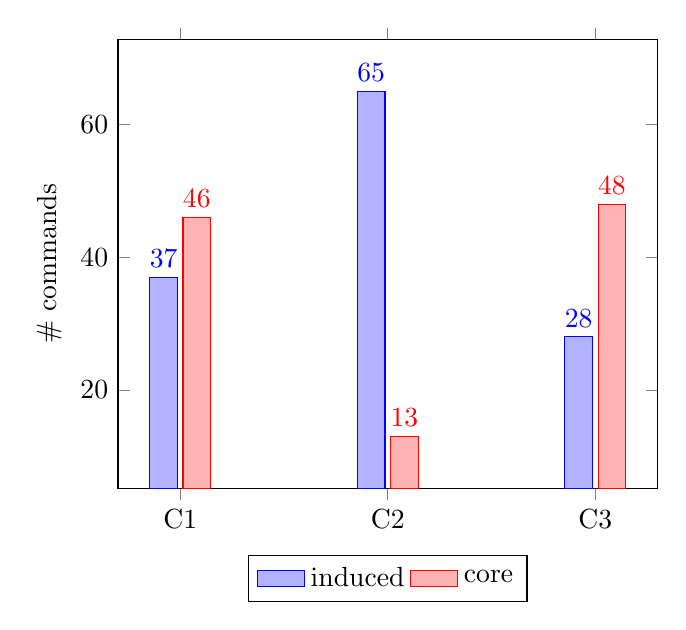
\begin{tikzpicture}
				\begin{axis}[
				    ybar,
				    area legend,
				    enlargelimits=0.15,
				    legend style={at={(0.5,-0.15)},
				      anchor=north,legend columns=-1},
				    ylabel={\# commands},
				    symbolic x coords={C1,C2,C3},
				    xtick=data,
				    nodes near coords,
				    ]
				\addplot coordinates {(C1,37) (C2,65) (C3,28)};
				\addplot coordinates {(C1,46) (C2,13) (C3,48)};
				\legend{induced, core}
				\end{axis}
				\end{tikzpicture}

	}
			}
\subfloat[][Using rules induced by others vs. self-induced rules]{\resizebox{0.5\linewidth}{!}{

				\label{fig:groupCRulesInducedBySelfVsOthers}
				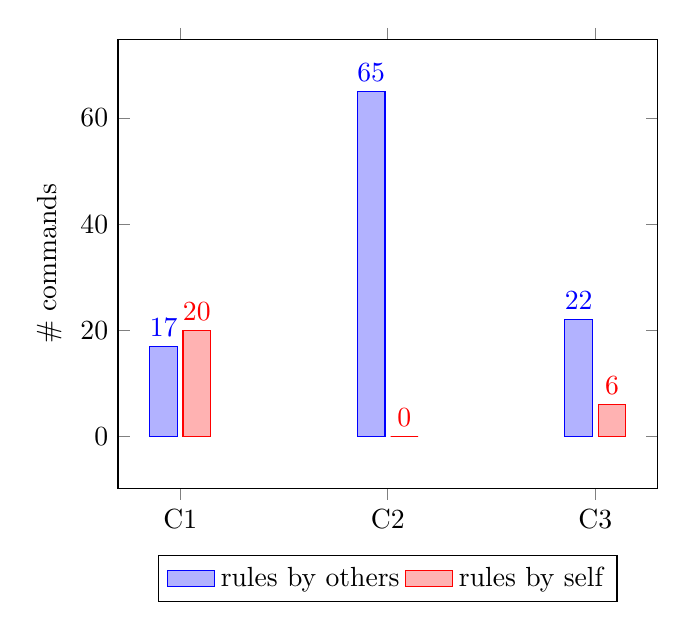
\begin{tikzpicture}
				\begin{axis}[
				    ybar,
				    area legend,
				    enlargelimits=0.15,
				    legend style={at={(0.5,-0.15)},
				      anchor=north,legend columns=-1},
				    ylabel={\# commands},
				    symbolic x coords={C1,C2,C3},
				    xtick=data,
				    nodes near coords,
				    ]
				\addplot coordinates {(C1,17) (C2,65) (C3,22)};
				\addplot coordinates {(C1,20) (C2,0) (C3,6)};
				\legend{rules by others, rules by self}
				\end{axis}
				\end{tikzpicture}

	}
			}
	\caption{Usage of induced rules in group C}
\end{figure}

\addtolength{\textheight}{-12cm}   % This command serves to balance the column lengths
                                  % on the last page of the document manually. It shortens
                                  % the textheight of the last page by a suitable amount.
                                  % This command does not take effect until the next page
                                  % so it should come on the page before the last. Make
                                  % sure that you do not shorten the textheight too much.

%%%%%%%%%%%%%%%%%%%%%%%%%%%%%%%%%%%%%%%%%%%%%%%%%%%%%%%%%%%%%%%%%%%%%%%%%%%%%%%%



%%%%%%%%%%%%%%%%%%%%%%%%%%%%%%%%%%%%%%%%%%%%%%%%%%%%%%%%%%%%%%%%%%%%%%%%%%%%%%%%



%%%%%%%%%%%%%%%%%%%%%%%%%%%%%%%%%%%%%%%%%%%%%%%%%%%%%%%%%%%%%%%%%%%%%%%%%%%%%%%%



%%%%%%%%%%%%%%%%%%%%%%%%%%%%%%%%%%%%%%%%%%%%%%%%%%%%%%%%%%%%%%%%%%%%%%%%%%%%%%%%


\section{Related work and discussion}
Wang et al.\cite{wangVoxelurn} present the idea of starting from a programming language and let users gradually naturalize it. They implement their system as a block world in which users can build various shapes of different colors. The changed setting of robot world introduces new challenges: language that contains declarative commands and unrealizable commands. Similar approach of learning from users in the context of personal assistants is presented in \cite{azariaLia}. Beltagy and Quirk\cite{beltagyIFTT} train a model (ensemble of neural network and logistic regression) that translates a task description from IFTTT dataset into executable representations. They show few ways to improve the performance, the most interesting of which is creating synthetic data by paraphrasing task descriptions. Work by Lin et al\cite{linTelina} has the similar motivation: starting with questions from popular programming-help websites that describe programmer's intention, they devise bash one liners accomplishing it. They use RNN to learn the structure of a command and k-NN algorithm for matching between entities and slots available in the structure. With an anticipated ubiquity of personal robots, there is a lot of work dealing with commanding robots or communicating with them as well as creating programming languages for robots usable by non-programmers. Alexandrova et al.\cite{roboFlow} created a flow-based visual programming language, balancing intuitiveness and expressivity. We believe that natural language - if done right - is the most promising interface towards robots (or machines in general). SHRDLU\cite{shrdlu} was a system that started the endeavor.  Kollar et al.\cite{kollarDialog} and Thomason et al.\cite{thomasonDialog} recognize the need for a dialog between a robot and a human in order for the robot to understand human's intentions. In \cite{kollarDialog} robot is able to learn the way humans refer to different tasks or locations. \cite{thomasonDialog} allows for learned objects to be compositions of existing objects (e.g.\  \emph{the office next to X's office}. In both cases robot is trying to fill-in the gaps in simple action patterns, navigation and delivery, and the actions can not be combined. The work by Kress-Gazit et al.\cite{hadasTranslatingStructuredEnglish},\cite{hadasLTLMop},\cite{hadasProvablyCorrectReactiveControlFromNaturalLanguage} focuses on translating natural language into LTL to bridge a gap from users to available formal methods tools. A robot is able to give an answer to what it is currently doing, based on the natural language to LTL translation tree, as well as explain why an action in unrealizable. The set of things a robot can understand is limited to implemented semantic behaviors. Tellex et al.\cite{tellexGrounding} solve the problem of grounding utterances from the command to objects in space by introducing a hierarchical structure that connects (indeed similar) expressions such as \emph{beside the truck} and \emph{beside the box}. Paul et al.\cite{paulGrounding} solve the same problem, but supports abstract expressions such as \emph{first cube in the second row}. These two lines of work are connected in \cite{boteanuVerifiableGrounding} - there the grounding problem is put in the context of reactive temporal commands and potential groundings. \par In this work we showed that the idea of naturalizing existing programming language is perfectly suited for the problem of communicating with robots. That's been a long-standing open research problem. Many suggested solutions struggle with a lack of expressivity and a lack of extensibility to the concepts natural to humans. The results showed in this paper give hope that a formal language for commanding robot could be - by community effort - turned into \emph{domain specific natural language}. To accomplish this, few improvements are needed: lowering the entry bar to the system in its early phase (currently, the bar is learning the core language), providing better programming tools to make the system more usable (explanations for unparseable utterances, better depiction of two offered meanings of an utterance that have the same execution, auto-complete for available pre-defined concepts...), and further increasing of system's precision. Furthermore, significant improvements could be gained by implementing standard NLP techniques (lemmatization, rephrasing of definition heads, rephrasing of initial formal grammar) on top of the naturalization process


\bibliography{relatedWorkList}
\bibliographystyle{ieeetr}



\end{document}
